%!TEX encoding = UTF-8

\chapter{Motivation and Scope of the Thesis}
\label{chap:motivation}

In recent years, it is becoming increasingly common to use robots in domestic and public spaces. The total number of professional service robots sold in~2016~(i.e., non-industrial robots) rose considerably by~24\% to~\num{59706} units, up from~\num{48018} in~2015, with similarly positive forecasts expected for the period until~2020\footnote{Executive Summary World Robotics~2017 Service Robots, \url{http://www.ifr.org/service-robots/statistics/}}.
When deployed in domestic and public environments, robotic machines are expected to take on roles such as personal home assistants, receptionists, waiters, couriers, and more.
It is now feasible, though not without problems, to think of social robots being located in the same physical areas as a person.
This societal shift bears the issue of how to make robots that work effectively alongside humans.
In other words, how to build robots that possess the capabilities~(e.g., perception, reasoning, action) to execute their tasks well, and that in doing that are robust and reactive to uncertainty~(e.g., noisy measurements) and unexpected events~(e.g., failures), and that collaborate with us adequately by assisting our activities, without being a costly encumbrance in terms of money, time, or patience.
Public scenarios require interfaces that are easy to use for the general public, including for special groups like disabled, elderly or technology challenged people.
Human users should be able to provide instructions to robots in a natural and effortless way, mainly with verbal language and with nonverbal communication~(e.g., with body gestures), but this task has not been attained in general.
This thesis contributes to bridging the usability gap that human users face when dealing with robots.

One of the open challenges in designing robots that operate successfully in the \emph{unpredictable} human environment is how to make them able to foresee what actions they can perform onto objects of the world, and what the effects of these actions will be: in other words, how to provide them with the ability to perceive object \emph{affordances}~(action possibilities), a concept originally introduced in the field of developmental psychology in the 1960s, and of increasing importance in robotic research~(see Fig.~\ref{fig:num_papers:aff}). \label{aff_definition}
First proposed by J.~Gibson~\cite{jgibson:2014}, an affordance is defined as: ``a resource that the environment offers any animal that has the capabilities to perceive and use it''.
Later, E.~Gibson studied the role of affordances and learning in children~\cite{egibson:2003:ep}, reflecting on ``discovering the information that specifies an affordance''.
These theories stress how \emph{interacting} with the environment~(i.e., acting on it with a body) and \emph{perceiving} the environment~(i.e., sensing relevant features and changes of the world) are interconnected and related.

Suppose that a robotic agent has to operate in an environment, in particular having to see and use the objects that are available in order to achieve a given goal, such as adding sugar to a coffee~(\emph{stirring the coffee}) in the presence of a cup with coffee, of a sugar bowl, and of a spoon~(ignoring, for simplicity, the aspect of how the goal was entered into the system by a human user).
Classical \ac{AI} and robotic systems~\cite{russell_norvig:ai3,siciliano:2016:handbook2} will permit the agent to achieve the goal, relying on perceptual sensing algorithms, symbolic planning, and robot manipulator control, \emph{provided that the objects are recognized correctly}, meaning that the ``ingredients'' needed for the task~(e.g., cup, bowl, spoon) have been previously learned by the system at training time, and are detected at testing time.
However, what happens when a spoon is not available, or its appearance and shape are considerably different from the spoons that the system was taught?
Classical \ac{AI} may not be able to cope with this scenario, whereas the incorporation of affordances can help filling in the gaps in the following sense.
Reasoning on the affordances of the objects gives the benefit of relying on the knowledge about an object's \emph{functional features} or sub-parts, rather than on knowing the object's name or identity.
In the coffee example, if no spoon is available, the agent could use another type of cutlery which is long and thin, but if even that is not available, it might use yet another object that would help stir the coffee~(e.g., an object with a thin and elongated shape, as in the upper part of Fig.~\ref{fig:two-streams_cv}).
Affordances are mental shortcuts for accessing properties of objects that lead to a goal-directed action, without having to explicitly recognize the object name or type.
Therefore, affordances are a means to \emph{generalization} in robotic perception.
\label{coffee_example}

A similar argumentation can be made when we consider instructions provided by a human user to another agent~(human or robot).
In interactions, too, \emph{objects carry key information} about the action, which is conveyed explicitly or implicitly.
Humans can instruct other agents to perform operations on objects by saying their explicit name out loud~(using a shared verbal language which is understood by partners), or by referring to their distinctive features in an ambiguous situation~(e.g., by saying ``the large green box''), or by pointing at the objects themselves~(using a shared nonverbal gesture while communicating with an interaction partner).
Interestingly, when a person makes a gesture that points in the direction of an object, a system can reason on the affordances of the pointed object, which is useful for \emph{action prediction}~(i.e., predicting what the person will do next, or intends to do).
Indeed, when a person refers~(in whichever way) to an object, they are often really referring to the useful properties of it.
All in all, we can summarize these examples by saying that an object can act as a \emph{mediator for interaction}.
\nopagebreak[1]
Affordances are one way to exploit this power.
\label{action_prediction}

\begin{figure}[t!] % force footnote to appear on same page
\centering
\subfloat[][Number of published papers including ``affordances'' and ``robots'' in their text.]
{ \includegraphics[width=0.45\textwidth]{num_papers_aff} \label{fig:num_papers:aff} } \quad
%
\subfloat[][Number of published papers including ``gestures'' and ``robots'' in their text.]
{ \includegraphics[width=0.45\textwidth]{num_papers_gest} \label{fig:num_papers:gest} } \\
%
\subfloat[][Number of published papers including the sentence ``\hri'' in their text.]
{ 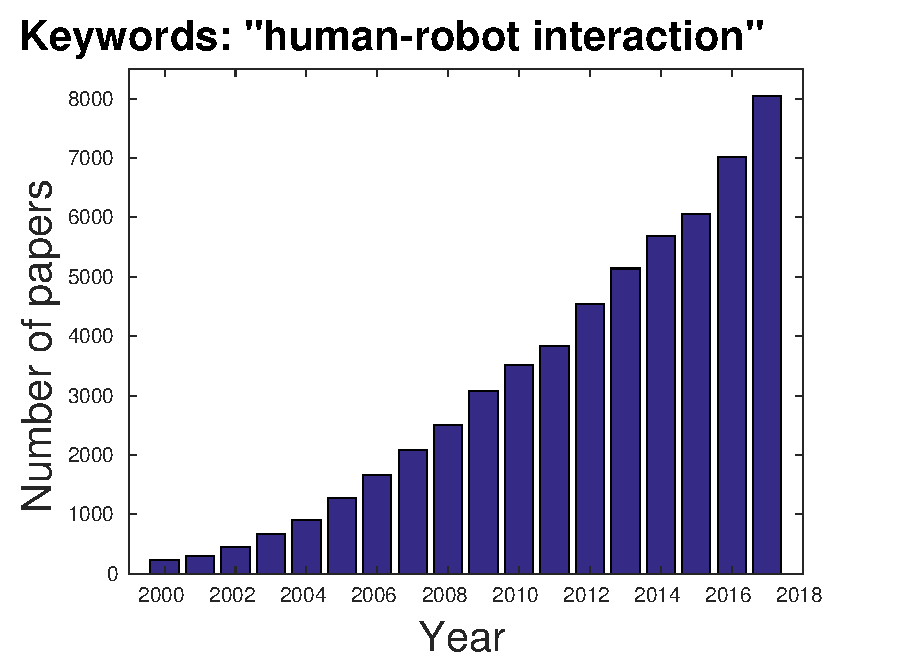
\includegraphics[width=0.45\textwidth]{num_papers_hri_in_quotes} \label{fig:num_papers:hri_in_quotes} } \quad
%
\subfloat[][Number of published papers including all of the keywords ``affordances'', ``gestures'', ``\hri'' and ``robots'' in their text.]
{ 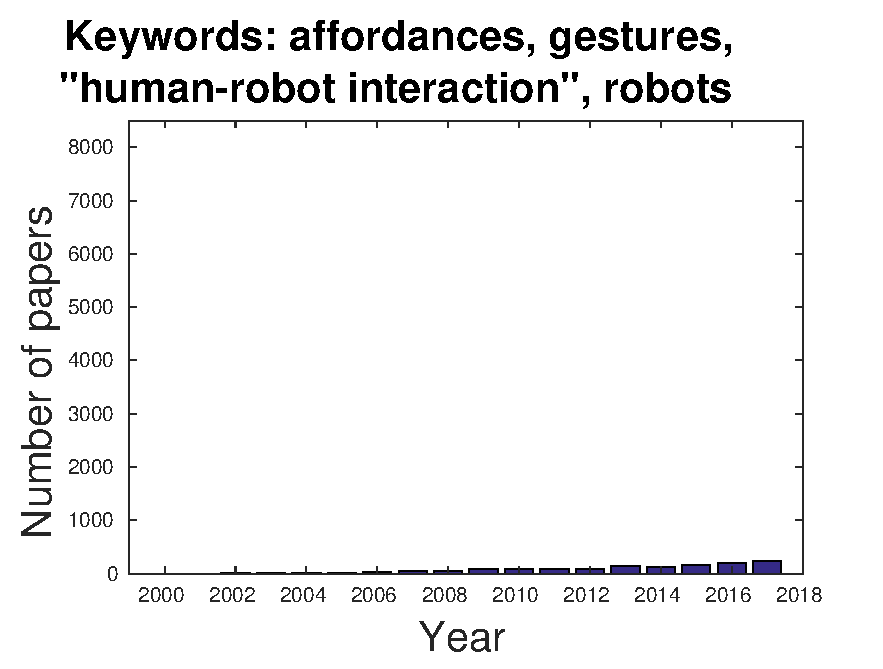
\includegraphics[width=0.45\textwidth]{num_papers_all} \label{fig:num_papers:all} }
% \cprotect protects \verb
% footnote within caption, https://tex.stackexchange.com/a/67030
\cprotect\caption[Number of published papers including relevant thesis keywords over time.]{Number of published papers including relevant thesis keywords over time. The searches in Fig.~\ref{fig:num_papers:aff}--\ref{fig:num_papers:hri_in_quotes} show a growing trend in terms of number of publications for individual topics, however Fig.~\ref{fig:num_papers:all} reveals that not many papers address all the considered topics jointly.
Plots computed from Google Scholar data, using the \verb!academic-keyword-occurrence! script by Volker Strobel\protect\footnotemark.}
\label{fig:num_papers}
\end{figure}
\footnotetext{\url{http://doi.org/10.5281/zenodo.1218409}}

Within robotic research, in addition to a growing interest in affordances as mentioned above, there has been a similar trend in topics such as body gestures~(see Fig.~\ref{fig:num_papers:gest}) and, in general, in \hri{} systems and studies~(see Fig.~\ref{fig:num_papers:hri_in_quotes}).
However, there are not many papers yet that address these topics \emph{jointly}, as seen in Fig.~\ref{fig:num_papers:all}: the number of published papers which mention all of the keywords~(in the entirety of the article text, not only in the title) ranges between~3 in year~2000 and about~180 in~2016.
Even though~180 papers is a reasonable number, it still constitutes a relatively small fraction of the whole body of articles produced by the robotics community yearly.

\section{Objectives}

This thesis revolves around the usefulness of affordances in robots, and the possible \emph{advantages of using robot affordances in conjunction with other modalities, such as human body gestures and language, for supporting effective interactions between humans and robots}.
The core goal is to develop computational models to use affordances and other environment elements in order to close the gap between human and robot knowledge.
We research how object affordances can provide a \emph{joint reference} between human and robot for the correct interpretation of gestural instructions, and how this can ultimately lead to intuitive robot utilization for the general population.
In particular, this work stems from the observation that objects contain important links to physical actions and action understanding when interacting with other agents.
From this idea, we develop a theory comprising objects affordances, body gestures and probabilistic inference.
We contribute software programs that can be deployed on real robotic systems.
We show a number of practical contributions in robot algorithms that incorporate the above concepts.

By advancing action recognition capabilities in robots through the combination of gestures and affordance perception, we also \allowbreak endow \allowbreak robots with the ability to recognize human actions during their enactment, i.e., before said actions are completed in their entirety.
The advantage is to provide robots the ability to \emph{anticipate} human actions and intentions, given contextual circumstances.
We show this anticipatory behavior and capability in \hr{} collaborative tasks, relying on the information provided by objects affordances, body gestures and probabilistic inference.

\begin{figure}
    \newcommand{\myscaleaffmodels}{0.45}
    \centering
    \subfloat[][Computational model of robot affordances by Montesano~\cite{montesano:2008}, explained in Ch.~\ref{chap:background}.]
    { \begin{tikzpicture}[scale=\myscaleaffmodels, every node/.style={transform shape}]
      \montesanoAE
      \montesanoO
      \end{tikzpicture} \label{fig:aff_models_intro:montesano}
    } \quad
    %
    \subfloat[][Computational model of affordances with associated verbal descriptions, by Salvi~\cite{salvi:2012:smcb}, explained in Ch.~\ref{chap:background}.]
    { \begin{tikzpicture}[scale=\myscaleaffmodels, every node/.style={transform shape}]
      \montesanoAE
      \montesanoO
      \salviW
      \end{tikzpicture} \label{fig:aff_models_intro:salvi}
    } \\
    %
    \hspace{-9cm} \footnotesize \emph{state of the art} \\
    \hrule
    \hspace{-9cm} \emph{our contributions} \normalsize \\
    %
    \subfloat[][Computational model of affordances with gestures and language, proposed in Ch.~\ref{chap:gestures}.]
    { \begin{tikzpicture}[scale=\myscaleaffmodels, every node/.style={transform shape}]
      \montesanoAE
      \montesanoO
      \saponaroGestRecBox
      \salviW
      \end{tikzpicture} \label{fig:aff_models_intro:gestures_lang}
    } \quad
    %
    \subfloat[][Computational model of affordances for dealing with multiple objects and tool use, proposed in Ch.~\ref{chap:tool}.]
    { \begin{tikzpicture}[scale=\myscaleaffmodels, every node/.style={transform shape}]
      \montesanoAE
      \saponaroManipulatorUseBox
      \end{tikzpicture} \label{fig:aff_models_intro:tools}
    }
\caption[Schematic diagrams of the cognitive robotic \allowbreak models discussed in this thesis.]{Schematic diagrams of the cognitive robotic models discussed in this thesis.
They all include a representation of affordances as relations between actions, objects and effects (Figs.~\ref{fig:aff_models_intro:montesano}--\ref{fig:aff_models_intro:tools}).
In addition, some of them include extensions or specific aspects being highlighted (Figs.~\ref{fig:aff_models_intro:gestures_lang}--\ref{fig:aff_models_intro:tools}).
Figs.~\ref{fig:aff_models_intro:montesano} and~\ref{fig:aff_models_intro:salvi} are prior existing works from the state of the art, whereas Figs.~\ref{fig:aff_models_intro:gestures_lang} and~\ref{fig:aff_models_intro:tools} are contributions of this thesis.}
\label{fig:aff_models_intro}
\end{figure}

Fig.~\ref{fig:aff_models_intro} illustrates the cognitive robotic models used in this thesis schematically.
Fig.~\ref{fig:aff_models_intro:montesano} exemplifies the state of the art in robot affordances: a computational implementation of simple object affordances, defined as the relations between actions, objects and effects, as proposed in the works of Montesano~\cite{montesano:2008}.
Fig.~\ref{fig:aff_models_intro:salvi} is also prior work from the state of the art, focusing on the joint learning of affordances and language descriptions.
Fig.~\ref{fig:aff_models_intro:gestures_lang} shows our contribution of incorporating gestures and language descriptions to the model, allowing a cognitive robot to reason about physical actions when external agents operate in an environment shared with the robot, to describe the scene verbally, and permitting anticipatory behavior.
Fig.~\ref{fig:aff_models_intro:tools} depicts our contribution related to tool use, which allow a robot to not only use a single object of the world, but to reason about the possibilities offered by a first grasped object (i.e., using a specific manipulator) onto a second object which is acted upon when the first one is in the agent's hand.

\bigskip

In the following sections, we present the constituent theoretical components upon which this thesis is based.
Sec.~\ref{sec:motivation:devrob} defines the principles that guide the framework of developmental robotics,
Sec.~\ref{sec:motivation:affordances} illustrates the concept of affordances and the advantages that it provides in robotics, and
Sec.~\ref{sec:motivation:neuro} specifies the neuroscience theories which are linked to our research.
Finally, Sec.~\ref{sec:motivation:main_contributions} lists the main contributions of the thesis, and Sec.~\ref{sec:motivation:outline} gives a brief outline of the structure of the next chapters.

\section{Developmental Robotics}
\label{sec:motivation:devrob}

Developmental robotics, also known as epigenetic robotics or ontogenetic robotics, is a subfield of robotics whose main aims are (i)~modeling the development of \emph{increasingly complex cognitive processes}~(for example, the understanding of language, or the acquisition of manipulation skills), and also (ii)~understanding how such processes emerge through physical and social interaction~\cite{lungarella:2003:devrobsurvey,cangelosi:2015:devrobbook}.
Developmental robotics takes direct inspiration from the progressive learning phenomena observed in children's cognitive development.
It is related to other fields such as \ac{AI}, developmental psychology, neuroscience and dynamical systems theory.

In this line of research, robots are used to verify theoretical models of emergence and development of action and cognition.
The rationale is the following: if a model is instantiated inside a system embedded in the real world, many things can be learned about its strengths and limitations.
Developmental robotics operates on short~(ontogenetic) time scales of single individuals, or small groups of individuals.
By contrast, evolutionary robotics typically operates on long~(phylogenetic) time scales and large populations of several individuals.

The basic idea behind developmental robotics~(i.e., that the mechanism of development can be used to understand and to construct cognition) can be traced back to Turing~\cite{turing:1950}:
``Instead of trying to produce a programme to simulate the adult mind, why not rather try to produce one which simulates the child's? If this were then subjected to an appropriate course of education, one would obtain the adult brain''.
Another core idea in developmental robotics is \emph{embodiment}~(or Embodied \acl{AI}), which states that intelligence~(e.g., common sense) can only be the result of learned experience of a body living in the real world~\cite{pfeifer:2006}.

This thesis follows the developmental robotics perspective: the contributions that we will describe in the next chapters hinge on the paradigm of a robot that learns about its surrounding environment by incremental \emph{self-exploration}, starting from a limited initial knowledge; in addition, this learning process is embodied, in the sense that it is conditioned on a particular, physical robot body~(e.g., the arms and hands can reach and manipulate certain objects and locations in the robot workspace, but not all of them).

\section{Motivation for Using Robot Affordances}
\label{sec:motivation:affordances}

Affordances, introduced in p.~\pageref{aff_definition}, correspond to action possibilities offered to agents by elements of the environment.
They can support service robotics\footnote{The \ac{ISO} defines a ``service robot'' as a robot ``that performs useful tasks for humans or equipment excluding industrial automation applications'' (ISO~8373).} and \hri{} applications for a number of reasons.

\begin{figure}
\centering
\includegraphics[width=0.9\textwidth]{door_handle.jpg}
\caption{A door handle affords the ability to be turned and pulled, resulting in the door to be open.}
\label{fig:door_handle}
\end{figure}

First, affordances are \emph{personal}: they depend on the agent~(or on the ``animal'', as in the original definition by J.~Gibson~\cite{jgibson:2014}).
For example, the door handle of Fig.~\ref{fig:door_handle} offers the affordance of being manipulated in order to open the door, but the precise motor realization of the act of turning the handle is different for an adult human or for a robot~(and also for other types of agents such as children or animals)~\cite{chemero:2003:outline,chemero:2007:gibsonian,jamone:2016:tcds}.
We can say that there is one set of affordances for humans and another one for robots.
Then, if a robot can understand both types, it can link human actions and robot actions.

Second, affordances are suited for learning and generalization behaviors on cognitive robots that manipulate objects of the world.
Modeling all the possible world interactions is unfeasible~(we cannot pre-program all the interactions between a robot, its motor action repertoire, and the resulting effects onto the objects of the world), therefore learning from experience is required.
However, to collect large amounts of robot sensorimotor data is challenging and costly.
Robot affordances are then one possibility to capture meaningful aspects of data, without necessarily requiring large amounts of data, but permitting to learn a model that can adapt to situations unseen during training.
We describe this aspect in Ch.~\ref{chap:background}.

Third, affordances can be profitably combined with \emph{communication}, both verbal~(i.e., language) and nonverbal~(i.e., gestures).
For example, the ability to foresee the action performed by other human agents onto physical objects is fundamental for successful \emph{anticipation} and collaboration in joint tasks.
If a robot can perceive the affordances offered to a human by objects present in a collaborative \hr{} scenario, it can monitor the evolution of the task, anticipate the final goal, and intervene in a timely manner.
We explore this aspect in Ch.~\ref{chap:gestures}.

Fourth, learning how humans operate \emph{tools} is crucial for having a robot operate in complex manipulation tasks that are typical in human-like environments.
We note that \emph{our hands are our first tools} in interacting with physical objects of the world; then, from~16~months of age, humans start developing functional tool use~\cite{fagard:2014:emergence}.
We investigate this transition on a humanoid robot, modeling the transfer from hand affordances~(i.e., perception of action possibilities offered by objects using different hand morphologies) to tool affordances~(i.e., perception of action possibilities offered by objects using different tools).
A robot can learn tool use capabilities in a gradual way, generalizing to different tools that afford different possibilities, similarly to how children progressively learn mutual interactions between different objects. Acquiring this capability permits a robot to perform actions that would otherwise not be possible, for example grasping a faraway object with the help of an elongated tool.
We explore these aspects in Ch.~\ref{chap:tool}.

Fifth, robot sensorimotor knowledge~(in the form of learned affordances) can be useful for symbolic reasoning in order to form a unified \emph{planning architecture} that allows a robot to carry out a complex manipulation task under challenging conditions and external disturbances~(e.g., noisy perception, motor problems, obstruction by other agents).
We present a case study about the POETICON++ project, which tackled all of those issues, in Ch.~\ref{chap:poeticon++_case_study}, introducing a robust action planning system that combines robot sensorimotor knowledge~(in the form of learned affordances) with symbolic reasoning, using a unified probabilistic representation.

\section{Neuroscience Inspiration}
\label{sec:motivation:neuro}

In this work we draw inspiration from neuroscience~(the science that deals with the function and structure of the nervous system and brain), in particular from the following concepts:
two-streams hypothesis; \allowbreak
canonical neurons and mirror neurons.
We will now briefly explain these ideas.

\subsection{Two-Streams Hypothesis}
\label{sec:motivation:neuro:twostreams}

\begin{figure}
\centering
\includegraphics[width=0.9\textwidth]{two-streams_hypothesis_brain}
\caption[Graphical illustration of the visual processing streams in the human brain according to the two-streams hypothesis.]{Graphical illustration of the visual processing streams in the human brain according to the two-streams hypothesis.
The ventral stream~(lower part of figure) is shown in purple, stretching from the visual cortex into the temporal lobe.
The dorsal stream~(upper part) is shown in green, stretching from the visual cortex into the parietal lobe.
Picture elaborated under the CC BY-SA~3.0 license from an image by Wikimedia user Selket, author of the original picture at \url{https://commons.wikimedia.org/wiki/File:Ventral-dorsal_streams.svg}.}
\label{fig:two-streams_brain}
\end{figure}

The \emph{two-streams hypothesis}~\cite{goodale_milner:1992,chao:2000:neuro} speculates that the primate cerebral cortex processes visual information using two separate pathways:
\begin{enumerate}
\item the ventral or ``what'' stream, responsible for object categorization and recognition;

\item the dorsal or ``where'' or ``how'' stream, which guides object-directed actions such as reaching and grasping.
\end{enumerate}

\begin{table}
\caption[Main differences between the ventral stream and the dorsal stream.]{Main differences between the ventral stream and the dorsal stream, adapted and simplified from~\cite{norman:2002:bbs}.}
\label{tab:two-streams_differences}
\centering
\begin{tabular}{lll}
\toprule
factor & ventral stream & dorsal stream \\
\midrule
function        & object recognition & visually-guided behavior \\
                &                    & (e.g., reaching and grasping) \\
sensitivity     & details (high      & motion (high temporal \\
                & spatial frequency) & frequency) \\
memory          & long-term storage  & short-term storage \\
speed           & slow               & fast \\
consciousness   & high               & low \\
reference frame & object-centered    & viewer-centered \\
                & (allocentric)      & (egocentric) \\
visual input    & foveal             & across all retina \\
\bottomrule
\end{tabular}
\end{table}

Fig.~\ref{fig:two-streams_brain} shows a graphical representation of the two streams in the human brain, whereas Table~\ref{tab:two-streams_differences} lists the main differences between the two pathways for the purpose of this thesis.
In particular, looking at the \emph{speed} characteristic~(i.e., speed of firing after receiving a visual stimulus), it has been observed that the ventral stream is relatively slow~\cite[p.~84]{norman:2002:bbs}, whereas the dorsal stream is faster~\cite{proverbio:2011:neuro}.
The dorsal pathway constitutes a direct, fast neural link~(\textasciitilde250~ms) between vision and motor activation areas in the human brain, bypassing other regions while performing tasks like object reasoning or recognition~\cite{tunik:2007:neuroimage}.
For example, when humans observe a small cup of coffee, they perceive the shape, the handle, and the action possibilities provided by that object (i.e., its affordances) through the fast dorsal stream, whereas the precise object classification provided by the slower ventral pathway does not have the same usefulness, depending on the task.

\begin{figure}
\centering
\includegraphics[width=0.9\textwidth]{two-streams_hypothesis_cv}
\caption[Illustration of the two-streams hypothesis from a computer vision point of view.]{Illustration of the two-streams hypothesis from a computer vision point of view.
The ventral and dorsal pathways are highlighted, having different features and scopes.
The work developed in this thesis mainly focuses on the dorsal pathway and on learning visual affordances, which does not require to know the identity of objects as in the ventral pathway.
However, in Ch.~\ref{chap:poeticon++_case_study}, we also show a case study that employs both types of object reasoning in parallel~(ventral and dorsal).}
\label{fig:two-streams_cv}
\end{figure}

The reason why this neuroscience theory can be fruitful for cognitive robotics is exemplified by looking at Fig.~\ref{fig:two-streams_cv}.
Each of the two streams has its own perceptual process~(with extracted features and outputs), depending on the intended application being considered.
In the case of the ventral stream, the application is typically object recognition: that is, identifying the label or name of objects present in the input image, provided that object classes have been previously learned by the system during a learning phase.

On the contrary, in the case of the dorsal stream, we seek visual object features that can be linked to functional properties of the object~(i.e., its affordances), without having to recognize the label of the object, that is, without having necessarily seen that object before.
Therefore, in the works reported in this thesis we rely on the dorsal stream type of reasoning, because it is a suitable model for \emph{reasoning on objects in a category-independent way}~(i.e., not focusing on the object name or category, but rather on its sub-parts and functional features).
To that end, we investigate the generalization capabilities provided by this type of reasoning~(e.g., when testing objects different from the ones seen during the training phase).
This dorsal pipeline is a complement to the ventral one, responsible for object recognition and categorization, which is a topic of its own in computer vision, outside the scope of this thesis.
However, in Ch.~\ref{chap:poeticon++_case_study}, we will show how it is possible and profitable to employ both types of object reasoning~(ventral and dorsal) in a scenario that involves \hri{} through spoken verbal requests by the human, action planning and manipulation by the robot.

All in all, we show how learned affordance skills can be leveraged by robots in several contexts and modalities: reasoning on tools, on hand postures, on human gestures, language, and for action planning during manipulation tasks.

\subsection{Canonical Neurons and Mirror Neurons}
\label{sec:motivation:neuro:canonical_and_mirror}

Certain classes of neurons have been observed to be active in primates~(apes and humans) not only during the execution of behaviors, but also during the perception of the objects that are related to these behaviors~\cite{rizzolatti:2004:arn}.

\emph{Canonical neurons} respond both during grasping action execution, and when we simply view an \emph{object of a particular shape}~\cite[Ch.~19]{kandel:2000:principles}.
In other words, these neurons have sensory properties such that they respond to the presentation of objects on which we can perform an action~(e.g., grasping).
The grasping of objects needs to be informed by the shape of the object: for instance, we grasp paperclips differently than how we grasp oranges.
The sensory input is used to drive appropriate grasping gestures.
Canonical neurons are not assumed to be responsible for visual recognition: they just receive relevant input from areas involved in the processing of visual features.
We use this idea to link geometrical features, computed from the shape of visually segmented objects, to robot affordances~(Ch.~\ref{chap:background}).

\emph{Mirror neurons} respond to the motor actions of others.
More precisely, according to the \emph{mirror neuron system} theory, there is a neurophysiological mechanism in the brain resulting in certain neurons firing in two different situations:
(i)~when performing a movement, or
(ii)~when sensing that a peer is performing a goal-directed movement~\cite{kilner:2009:jneurosci}.
The interpretation is that sensing and execution of movement are two sides of the same coin, and this mirroring mechanism is a fundamental part of action understanding and imitation learning skills~\cite{fogassi:2005:science,gazzola:2007:neuroimage}.
We use this idea to recognize manipulative gestures performed by external agents~(Ch.~\ref{chap:gestures})
and reasoning about the functional properties of the objects involved,
thus exploring action prediction and action anticipation capabilities~(as in the pointing gesture example of p.~\pageref{action_prediction})
integrating affordances with gestures.

People have an \apriori{} knowledge about others' body parts, and they use movement cues to understand what actions or gestures are being executed by others.
This mechanism can be replicated on a robot, encoding a gesture as the union of (i)~body part (appearance cue) and (ii)~movement.
We can interpret others' actions because what others do belongs to our motor repertoire or experience~\cite{rizzolatti:2001:nrn}.

\bigskip

To summarize, the contributions described in this thesis are based on a model of the environment surrounding the robot, with the novelty of representing the knowledge of this environment with affordances, beyond the mere recognition of specific objects.
Thus, our model looks at the physical objects present in the scene, their affordances, as well as people with their informative body gestures and actions.

\section{Contributions}
\label{sec:motivation:main_contributions}

The main contributions of this thesis are:
\begin{itemize}
\item a framework for visual robot affordance learning, based on autonomous robot exploration of the world, sensorimotor data collection and statistical models~(\aclp{BN}).
This system was implemented over the years 2010--2018 as a modular software to be deployed on humanoid robots, focusing on flexibility~(e.g., separating perception, learning and motor components, and allowing the user to employ some or all of them as needed) and real-time operations~(e.g., supporting robot cameras which capture images at~$30$ frames per second).
As a result, it was adopted as a building block for the further contributions of this thesis~(listed in the bullet points below), but it also had an impact externally, being adopted by other researchers: \cite{morse:2016:cogsci,dehban:2016:eccvws,dehban:2016:icra,dehban:2017:humanoids};

\item the combination of object affordances with communication (gestures and language).
This approach allows a robot to interpret and describe the actions of human agents by reusing the robot's previous experience.
This part produced the following publications:
\listPublicationsGestures

\item a model for tool use affordances in robots.
The main contributions were
(i)~the visual feature extraction component, capable of processing multiple objects simultaneously, extracting information both from the shape of whole objects as well as from their sub-parts;
(ii)~in the learning component, designing and evaluating various types of computational affordance models and parameters for assorted tasks (e.g., generalization to unseen objects; transfer of learned knowledge from a simulated robot to a real one);
(iii)~a method for learning the affordances of different robot hand postures, investigating the link from hand affordances~(i.e., action possibilities by using the hands) to tool affordances~(action possibilities by using tools).
This part produced the following publications:
\listPublicationsTools

\item a case study about the application of affordances and human verbal instructions for robot \emph{planning of manipulation tasks}, developed within the scope of the POETICON++ research project.
This part produced the following publications:
\listPublicationsPoeticonpp

\item an appendix that describes a novel human gesture recognition model for manipulative hand gestures, inspired by statistical techniques from \ac{ASR}.
It produced the following publication:
\listPublicationsAppendixGestureRecognition

\item finally, an appendix related to robot communication~(rather than robot perception and action, the core topics of the thesis):
the perceived social attitude attributed by non-technical users when observing certain head and body gestures performed by a robot.
This study paves the way for an active learning system capable of optimizing robot motion parameters with the aim of improving the communicative expressiveness.
It produced the following publication:
\listPublicationsAppendixHumanPercRobotGest

\end{itemize}

\section{Outline of the Thesis}
\label{sec:motivation:outline}

\begin{figure}
\centering
\includegraphics[width=0.9\textwidth]{chapters_diagram}
\caption{Structure of the thesis.}
\label{fig:chapters_diagram}
\end{figure}

The thesis is structured as sketched in Fig.~\ref{fig:chapters_diagram}.

Ch.~\ref{chap:background} illustrates
the main machine learning notation and concepts~(including \aclp{BN}) used in the thesis, and
the previous works in the literature which are related to our broad scope~(other chapters also contain specific related work sections).

Ch.~\ref{chap:platform} describes the experimental platform:
the iCub humanoid robot,
the experimental scenario under study, and
our modular software framework for robot affordance learning, focused on autonomous robot exploration of the world and visual processing, used as a building block in the rest of the thesis.

Ch.~\ref{chap:gestures} presents a computational model that combines affordances with language, broadly speaking.
It does that by incorporating
nonverbal language, in the form of \emph{human gestures}; and also
verbal language, by generating verbal descriptions of manipulative scenes.

Ch.~\ref{chap:tool} shows an affordance model that deals with multiple objects, giving rise to \emph{tool use}, including the link from hand affordances~(i.e., action possibilities by using the hands) to tool affordances~(action possibilities by using tools).

Ch.~\ref{chap:poeticon++_case_study} illustrates a case study about the application of affordances and human verbal instruction interpretation for robot \emph{planning of manipulation tasks}, developed within the scope of the POETICON++ research project.

Ch.~\ref{chap:final_remarks} draws the conclusions and lists the avenues for future work.

Appendix~\ref{chap:gesture_recognition} presents the details of the human gesture recognizer for manipulative hand gestures: this recognizer was inspired by statistical techniques from \ac{ASR}, and it was employed as one of the components of Ch.~\ref{chap:gestures},

Finally, as far as the robot communication aspect is concerned~(besides robot perception and action, the core topics of the thesis),
Appendix~\ref{chap:human_perc_robotgest} deals with the perceived social attitude attributed by non-technical users when observing certain body gestures performed by a robot.
